\documentclass{article}

\usepackage{graphicx}
\usepackage{tikz}
\usepackage{tikzsymbols}
\usetikzlibrary{calc,patterns,shapes.geometric}
\pagestyle{empty}
\usepackage[margin=0pt]{geometry}
\geometry{papersize={14in,12in}}

\def\centerarc[#1](#2)(#3:#4:#5){\draw[#1] ($(#2)+({#5*cos(#3)},{#5*sin(#3)})$) arc (#3:#4:#5);}

\begin{document}
	\begin{figure}
		\centering
		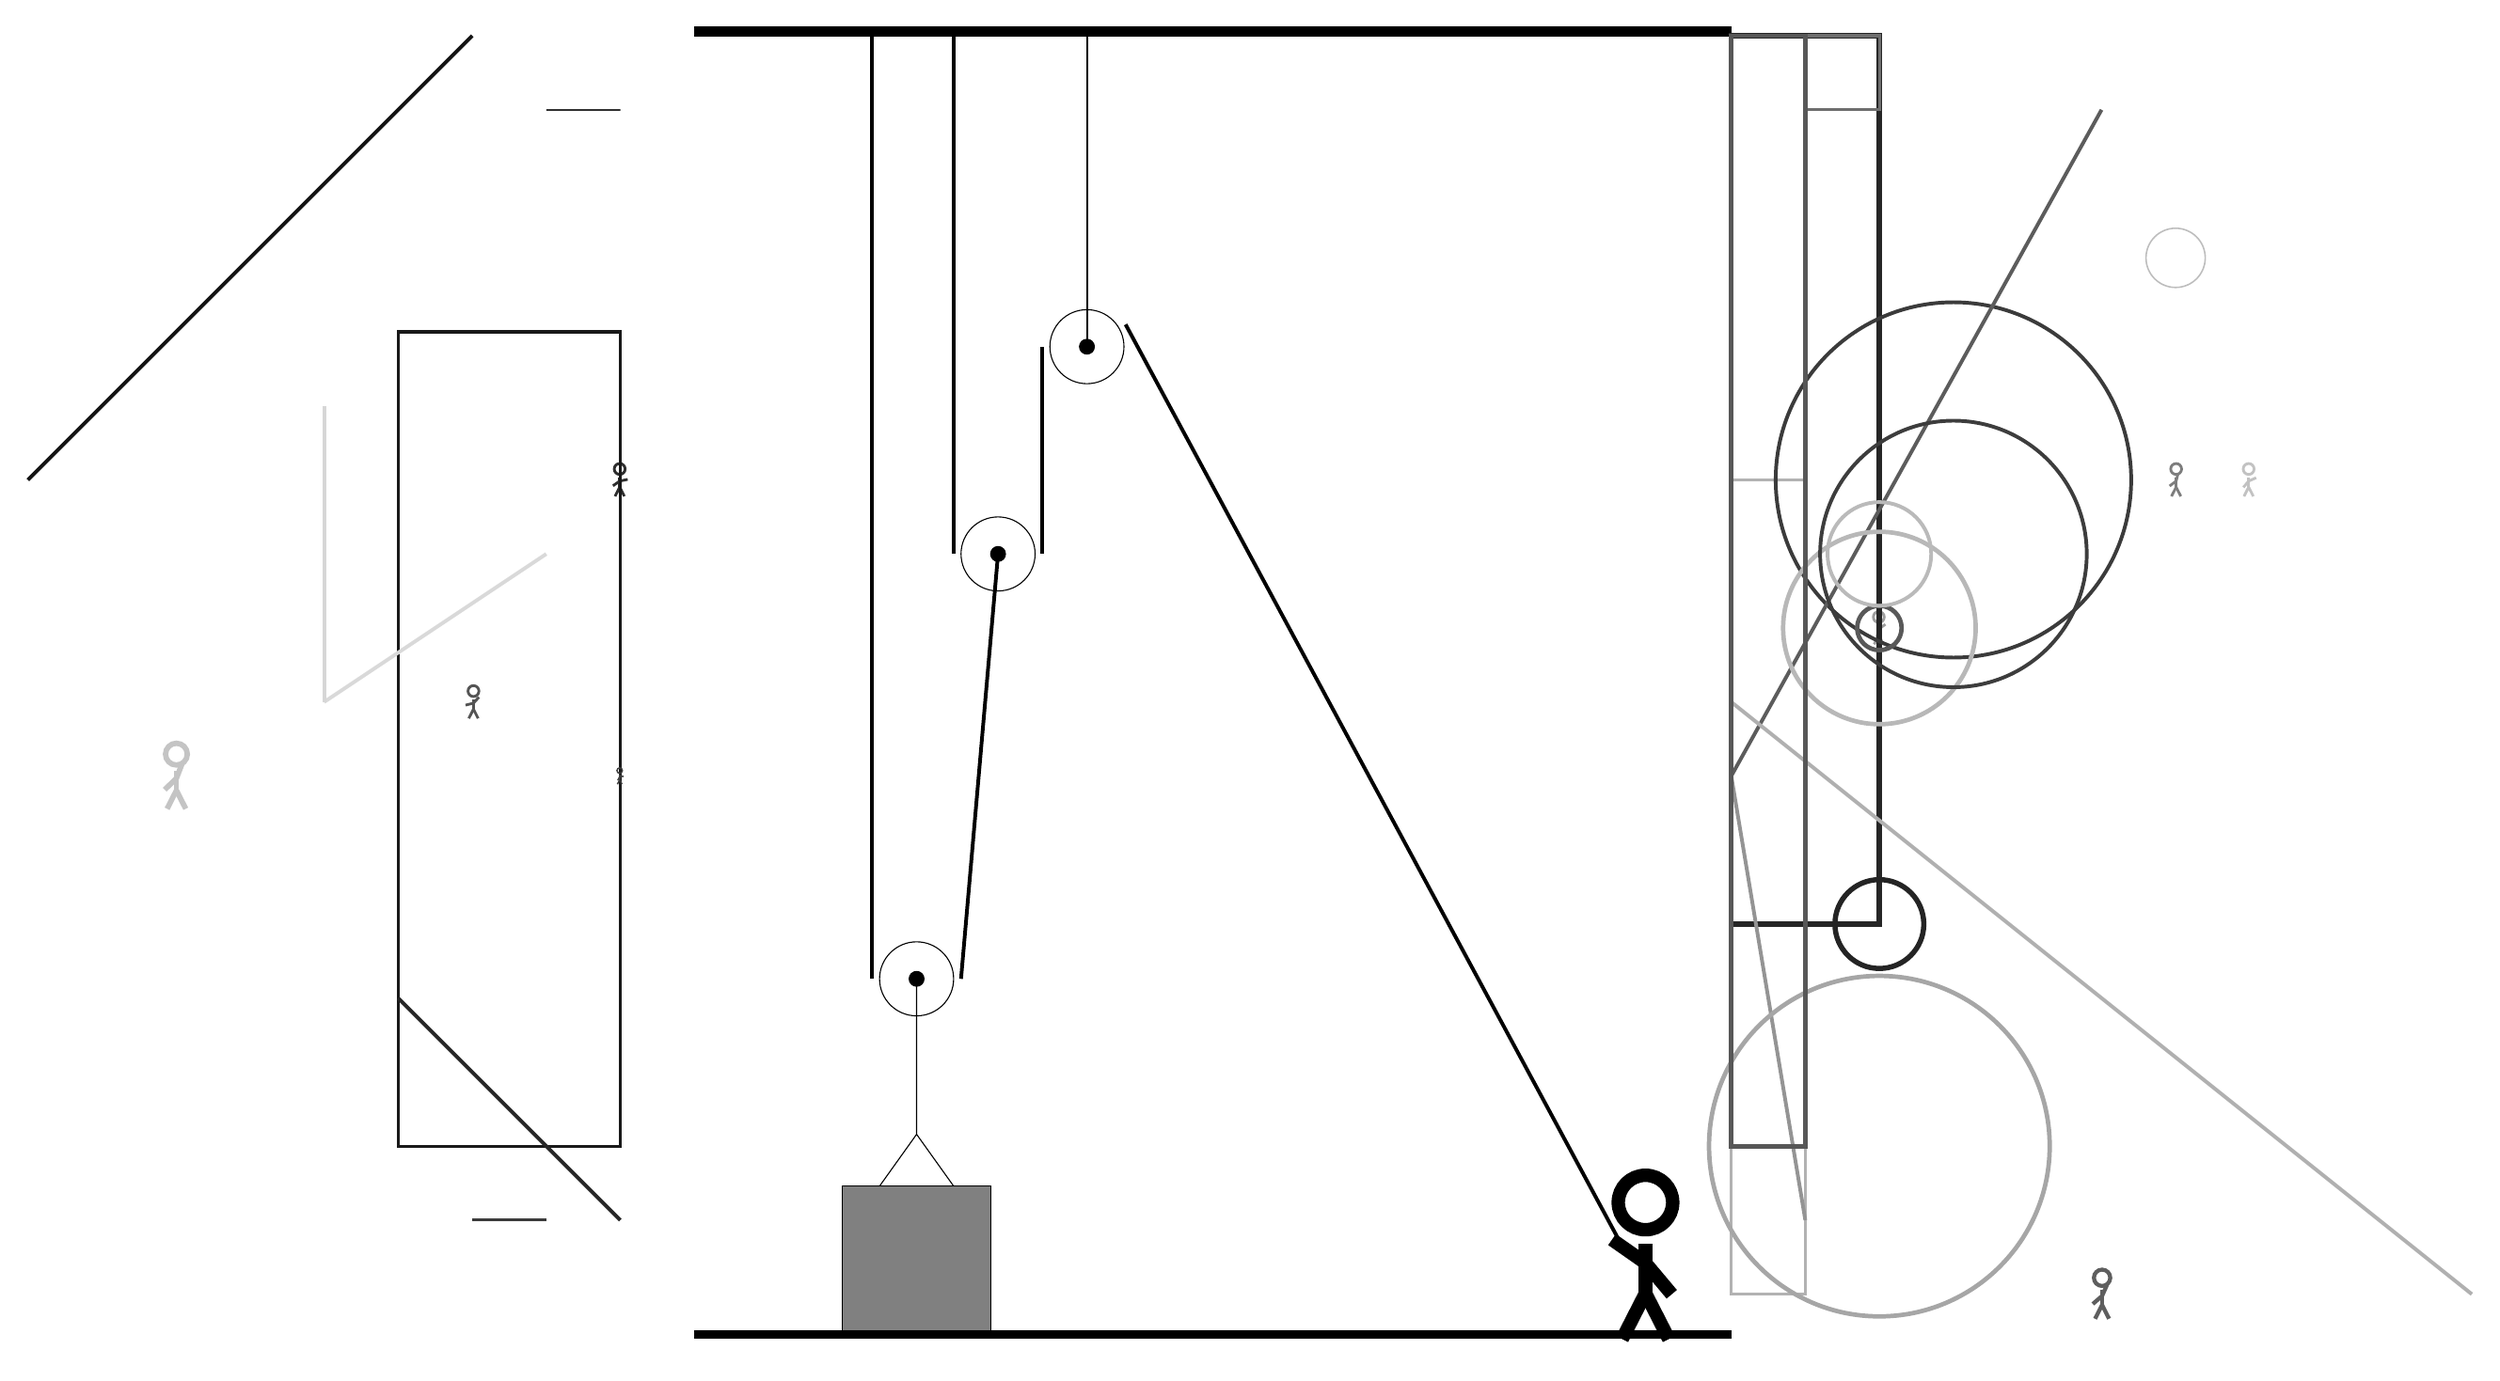
\begin{tikzpicture}
			%%%%% START %%%%%
			
			\draw[fill=black] (-2, 14) rectangle (12, 14.125);
			
			\draw (1, 1.26) circle (0.5);
			\draw[fill=black] (1, 1.26) circle (0.1);
			
			\draw (2.1, 7.0) circle (0.5);
			\draw[fill=black] (2.1, 7.0) circle (0.1);
			
			\draw (3.3, 9.8) circle (0.5);
			\draw[fill=black] (3.3, 9.8) circle (0.1);
			\draw[thick] (3.3, 9.8) -- (3.3, 14);
			
			\node[line width=0.4mm, color=black!82] at (-3, 8) {\Strichmaxerl[2][35][12]};
			
			\node[line width=0.3mm, color=black!38] at (14, 6) {\Strichmaxerl[2][77][36]};
			\node[line width=0.6mm, color=black!67] at (-5, 5) {\Strichmaxerl[2][14][48]};
			\node[line width=0.5mm, color=black!23] at (-9, 4) {\Strichmaxerl[4][44][69]};
			
			\draw[line width=0.7mm, color=black!85] (12, 14) rectangle (14, 2);
			\draw[line width=0.4mm, color=black!30] (13, 8) rectangle (12, -3);
			\node[line width=0.4mm, color=black!51] at (18, 8) {\Strichmaxerl[2][37][76]};
			
			\draw [line width=0.5mm, color=black!77](15, 8) circle (2.4);
			\draw[line width=0.5mm, color=black!64](17, 13) -- (12, 4);
			\draw[line width=0.5mm, color=black!42](12, 4) -- (13, -2);
			
			\draw[line width=0.4mm, color=black!90] (-3, 10) rectangle (-6, -1);
			\draw [line width=0.6mm, color=black!28](14, 6) circle (1.3);
			\draw[line width=0.4mm, color=black!77] (-4, -2) rectangle (-5, -2);
			
			\draw[line width=0.5mm, color=black!31](12, 5) -- (22, -3);
			\node[line width=0.2mm, color=black!24] at (19, 8) {\Strichmaxerl[2][50][24]};
			\draw[line width=0.2mm, color=black!81] (-4, 13) rectangle (-3, 13);
			
			\draw [line width=0.6mm, color=black!65](14, 6) circle (0.3);
			\draw [line width=0.6mm, color=black!35](14, -1) circle (2.3);
			\draw[line width=0.5mm, color=black!15](-4, 7) -- (-7, 5);
			\draw [line width=0.5mm, color=black!27](14, 7) circle (0.7);
			\node[line width=0.4mm, color=black!63] at (17, -3) {\Strichmaxerl[3][41][66]};
			\draw [line width=0.2mm, color=black!26](18, 11) circle (0.4);
			\draw [line width=0.5mm, color=black!76](15, 7) circle (1.8);
			\draw[line width=0.4mm, color=black!57] (13, 14) rectangle (14, 13);
			\draw [line width=0.7mm, color=black!86](14, 2) circle (0.6);
			
			\node[line width=0.2mm, color=black!76] at (-3, 4) {\Strichmaxerl[1][62][4]};
			\draw[line width=0.5mm, color=black!85](-6, 1) -- (-3, -2);
			\draw[line width=0.5mm, color=black!92](-5, 14) -- (-11, 8);
			\draw[line width=0.6mm, color=black!66] (12, 14) rectangle (13, -1);
			\draw[line width=0.5mm, color=black!16](-7, 5) -- (-7, 9);
			
			\draw (1, 1.26) -- (1, -0.84) -- (0.5, -1.54) -- (1.5, -1.54) -- (1, -0.84);
			\draw[fill=black!50] (0, -1.54) rectangle (2, -3.54);
			
			\draw[line width=0.5mm] (0.4, 14) -- (0.4, 1.26);
			\centerarc[line width=0.5mm](1, 1.26)(180:360:0.6);
			\draw[line width=0.5mm](1.6, 1.26) -- (2.1, 7.0);
			\draw[line width=0.5mm] (1.5, 14) -- (1.5, 7.0);
			\centerarc[line width=0.5mm](2.1, 7.0)(180:360:0.6);
			\draw[line width=0.5mm](2.7, 7.0) -- (2.7, 9.8);
			\centerarc[line width=0.5mm](3.3, 9.8)(30:180:0.6);
			\draw[line width=0.5mm] (3.822, 10.1) -- (10.5, -2.3);
			
			\node at (10.8, -2.5) {\Strichmaxerl[10][-35][-50]};
			
			\draw[fill=black] (-2, -3.5) rectangle (12, -3.6);
			
			%%%%% END %%%%%
		\end{tikzpicture}
	\end{figure}	
\end{document}